\chapter{評価}
著者らはTravelatARを用いて評価実験を行った.
\section{実験環境}
\figref{fig:env}に実験時の環境を\figref{fig:siten},\figref{fig:nonsiten}は被験者の視界を示す.
被験者は20代の男性6名である.
本システムでは道芝\cite{siba}にて,リアルテクスチャをアタッチしたバーチャル床をアニメーション重畳表示した場合と
Nonリアルテクスチャをアタッチしたバーチャル床をアニメーション重畳表示した場合
を比べてユーザの歩行速度制御に有位性が出るか否か調査する.
道芝の長さは20メートルとなっている.
今回使用するシステムでバーチャル床は,\figref{fig:maekara}のよう,ユーザに向かってくるよう動く.
被験者は頭にARグラスのHoloLens2を,体にはiPhone11 proを揺れないよう固定して装着してもらう\cite{holo}\cite{ipon}.
\begin{figure}[H]
    \centering
    \fbox{
        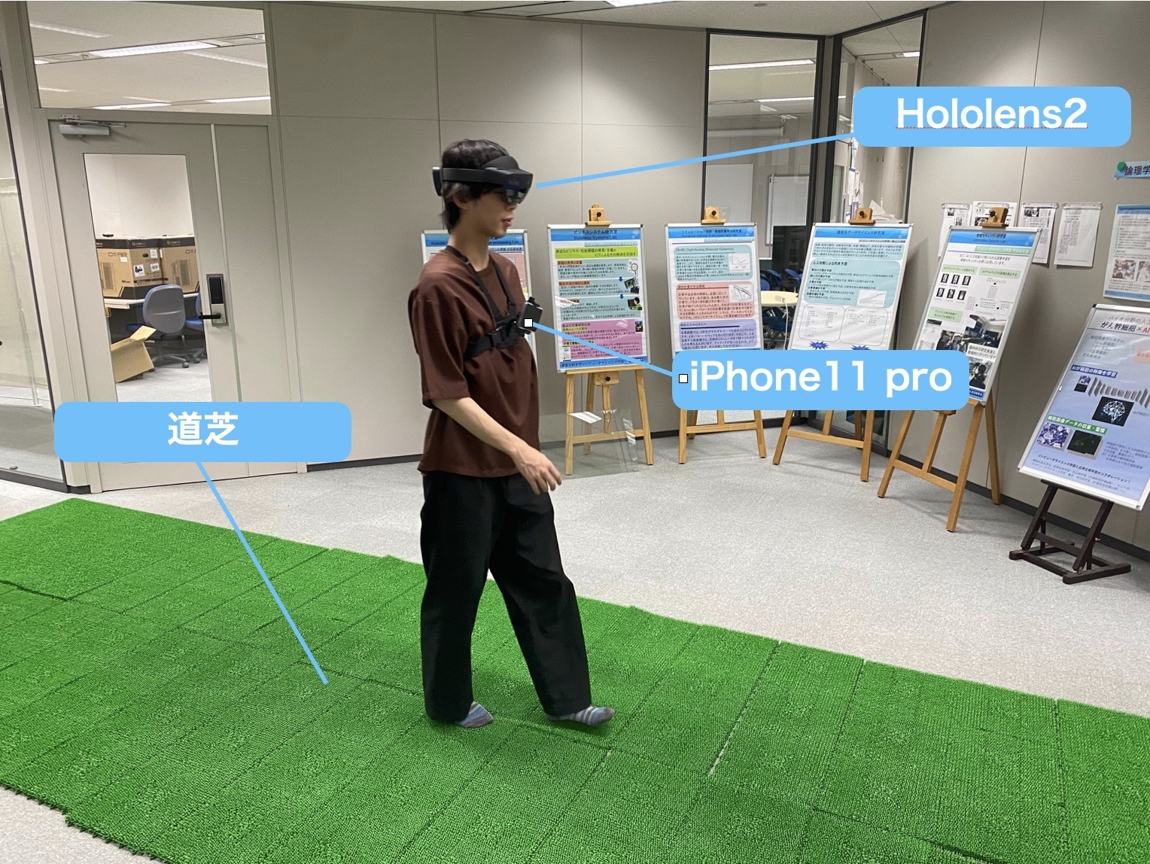
\includegraphics[keepaspectratio, width=0.6\linewidth]{fig/enviroment.png}
    }
    \caption{実験環境}
    \label{fig:env}
\end{figure}
\begin{figure}[H]
    \centering
    \fbox{
        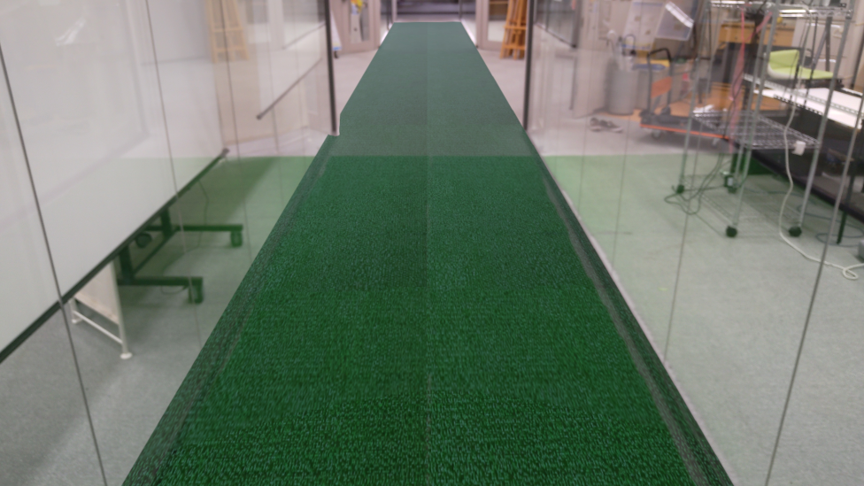
\includegraphics[width=0.8\linewidth]{fig/siten.png}
    }
    \caption{ユーザの視界(リアルテクスチャ適用)}
    \label{fig:siten}
\end{figure}
\begin{figure}[H]
    \centering
    \fbox{
        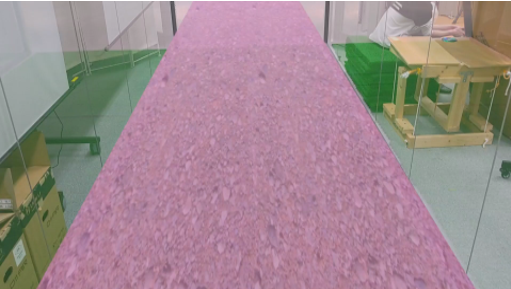
\includegraphics[width=0.8\linewidth]{fig/nonreal.PNG}
    }
    \caption{ユーザの視界(Nonリアルテクスチャ適用(5RP砂利))}
    \label{fig:nonsiten}
\end{figure}

\begin{figure}[H]
    \centering
    \fbox{
        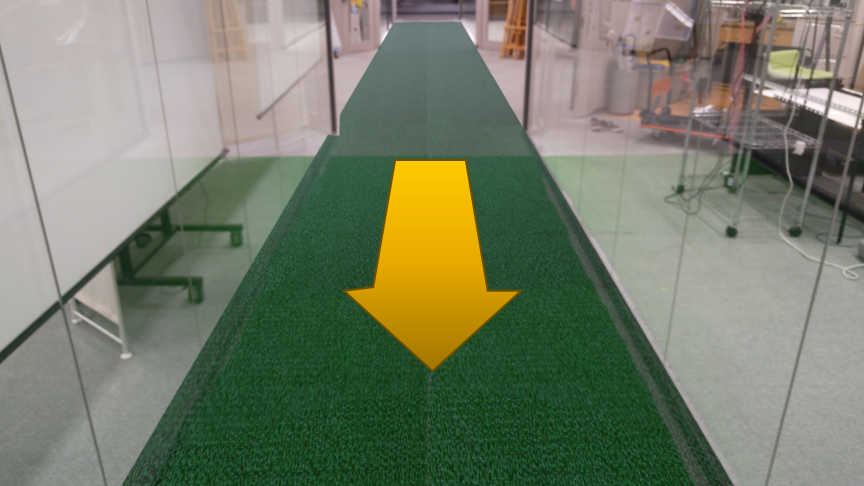
\includegraphics[width=0.8\linewidth]{fig/11.png}
    }
    \caption{本実験でのバーチャル床の動き}
    \label{fig:maekara}
\end{figure}

\section{実験手順}
実験手順を以下に示す.
\begin{enumerate}
    \item スタート地点に直立してもらった
    \item 被験者の装着しているiPhone11 proのセンサーのスイッチをオンにした
    \item 指定距離歩いてもらう
    \item 歩き終わった位置で直立してもらう
    \item センサーのスイッチをオフにする
\end{enumerate}
上記の手順を6回同じシステムで繰り返してもらい,それを1セットとした.
また,1セット終わるたびアンケートに回答してもらった.
この手順をシステムを使用していない状態のHoloLens2を装着した状態,
12種類の本システムを使用した状態の計13セット行ってもらった.



\section{評価方法}
本稿では定性評価と定量評価を行う.


定性評価では,酔いに関する主観的評価尺度であるThe Simulator Sickness Questionnaire((SSQ))\tabref{tab:SSQ}によるアンケートをとる\cite{ssq}.
その後,リアルテクスチャに関して,実際に床が動いているよう感じたかの他,
歩いている速度が早く感じるか,遅く感じるかといった感覚を速度感と定義して
システム未使用時に比べ,速い速度感を得たかと遅い速度感を得たかを
それぞれの1(まったく感じなかった)~5(非常に感じた)までの5段階のリッカート尺度を用いたアンケートを取る.
アンケートの最後には自由記述欄も用意した.
\begin{table}[h]
    \begin{center}
        \caption{The Simulator Sickness Questionnaire} \label{tab:SSQ}
        \begin{tabular}{c|l}\hline\hline
            質問番号 & 質問項目                                             \\\hline
            1        & 一般的な不快感がある                                 \\
            2        & 疲労感がある                                         \\
            3        & 頭痛がする                                           \\
            4        & 眼が疲れている                                       \\
            5        & 眼の焦点がぼける                                     \\
            6        & 唾液が増えている                                     \\
            7        & 発汗している                                         \\
            8        & 吐き気がする                                         \\
            9        & 集中できない                                         \\
            10       & 頭が重い                                             \\
            11       & 眼がかすむ                                           \\
            12       & (眼を開けた状態で)フラッとするようなめまい感がある \\
            13       & (眼を閉じた状態で)フラッとするようなめまい感がある \\
            14       & 自分や周囲が回転するようなめまいがある               \\
            15       & 胃の存在感がある                                     \\
            16       & げっぷが出る                                         \\\hline
        \end{tabular}
    \end{center}
\end{table}


定量評価では被験者の体に装着されたiPhone11 proの加速度センサー
を用いて歩行時間を計測し,評価する.
その際,以下の組み合わせごとに6回の「ゴールまで歩いた時間」の平均値を比べ,リアルテクスチャの有用性を評価した.
\begin{quote}
    \begin{itemize}
        \item システム無し・システム有(リアルテクスチャ)
        \item システム無し・システム有(11種類のNonリアルテクスチャそれぞれ)
    \end{itemize}
\end{quote}







\section{実験結果}

定性評価の結果を以下に示す.
\figref{fig:anke1}にシステム未使用時に比べ,速い速度感を得たか,
\figref{fig:anke2}にシステム未使用時に比べ,遅い速度感を得たか,
\figref{fig:anke3}にバーチャル床は本物の床が動いているように見えたかのアンケート結果を示す.
これらの棒グラフは,左から1(まったく感じなかった)~5(非常に感じた)となっている.
\figref{fig:anke1}から,色は人工芝の反対であり,模様も近似させていない5RP砂利がもっとも速い速度感を被験者に与えたことがわかった.
また,\figref{fig:anke2}からはほとんどのテクスチャが遅い速度感を与えなかったことがわかるが,5G天然だけは被験者によって意見が分かれている.
\figref{fig:anke3}から,リアルテクスチャである5Gは12種類のテクスチャの中で一番本物の床が動いているように見えたという結果を得た.
\begin{figure}[H]
    \centering
    \fbox{
        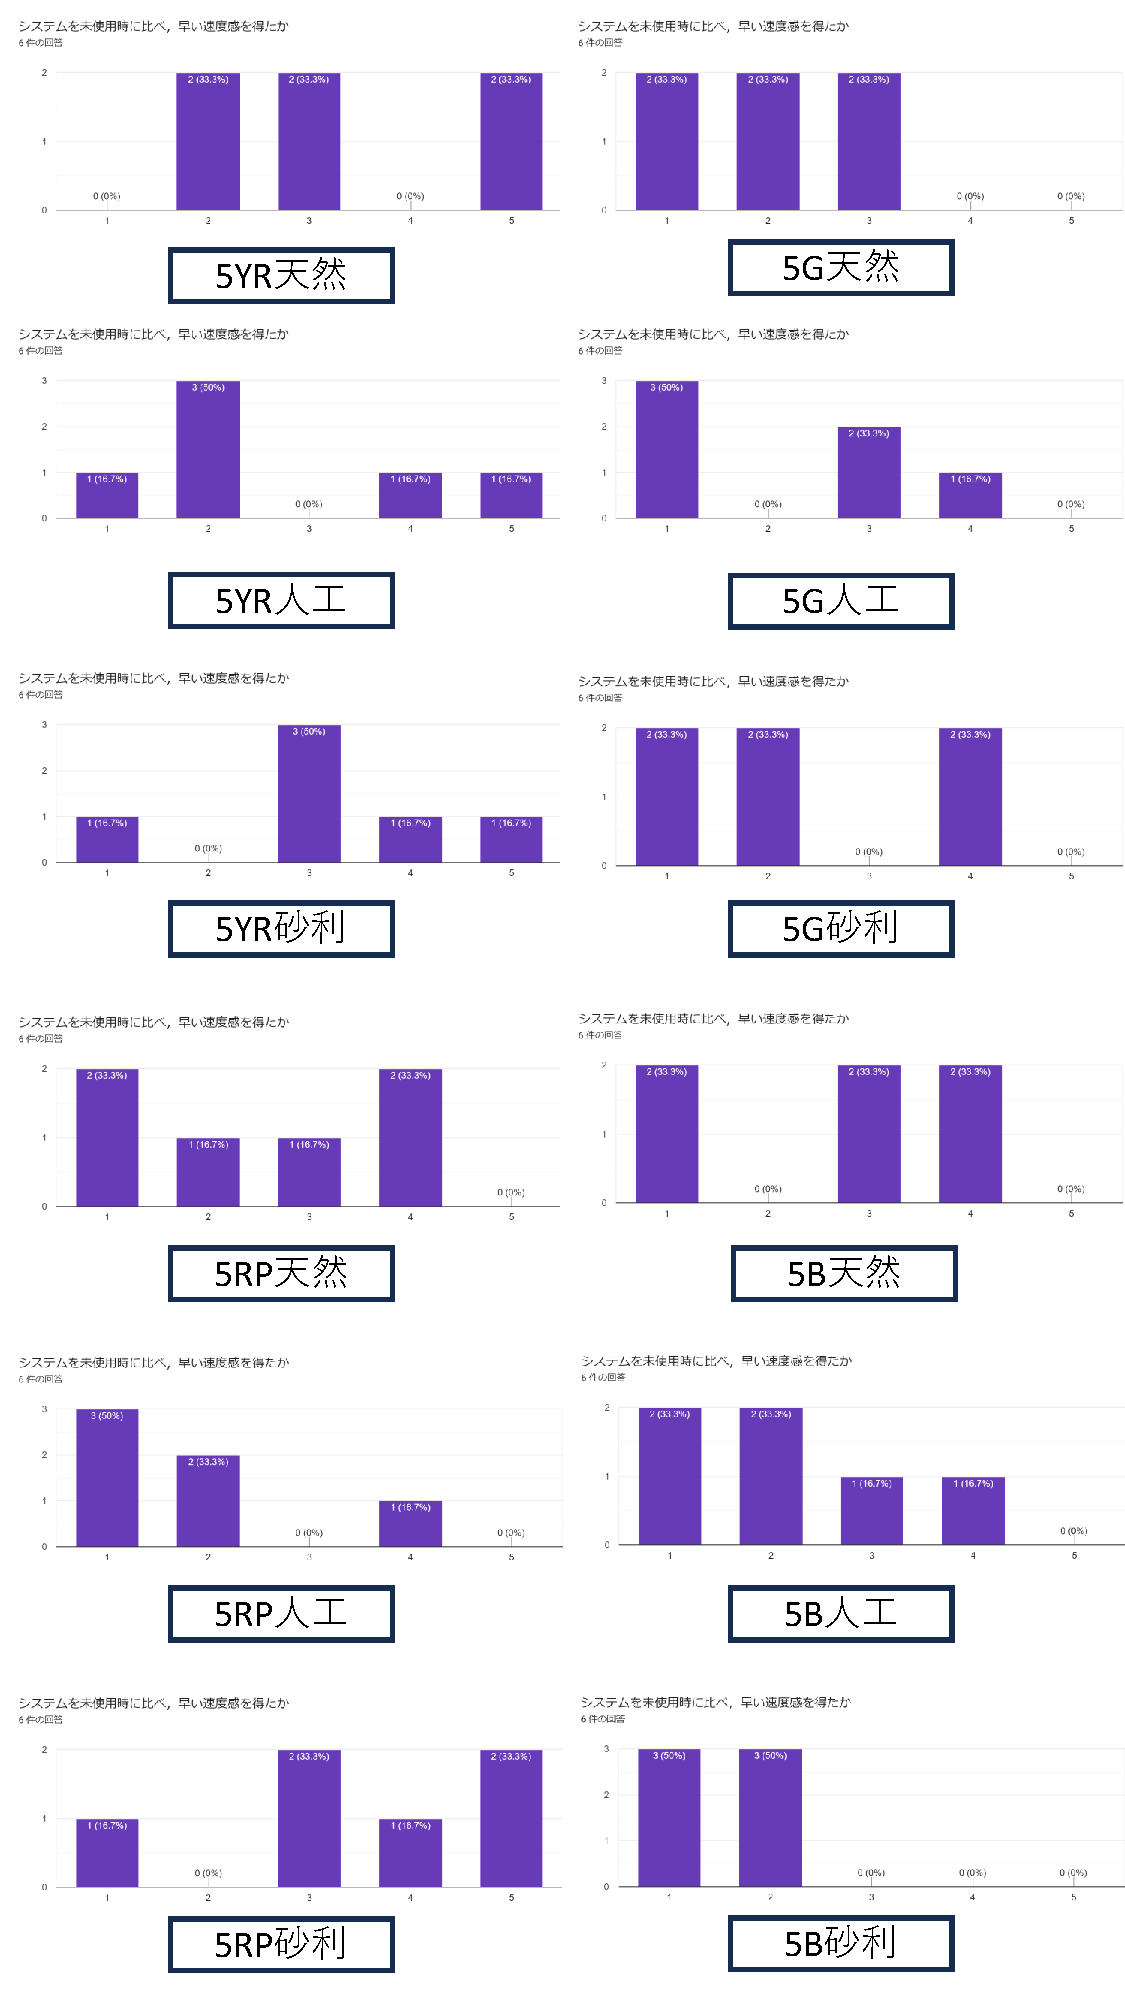
\includegraphics[width=0.7\linewidth]{fig/アンケート結果.pdf}
    }
    \caption{主観的な速度感に関するアンケート結果(上昇)}
    \label{fig:anke1}
\end{figure}

\begin{figure}[H]
    \centering
    \fbox{
        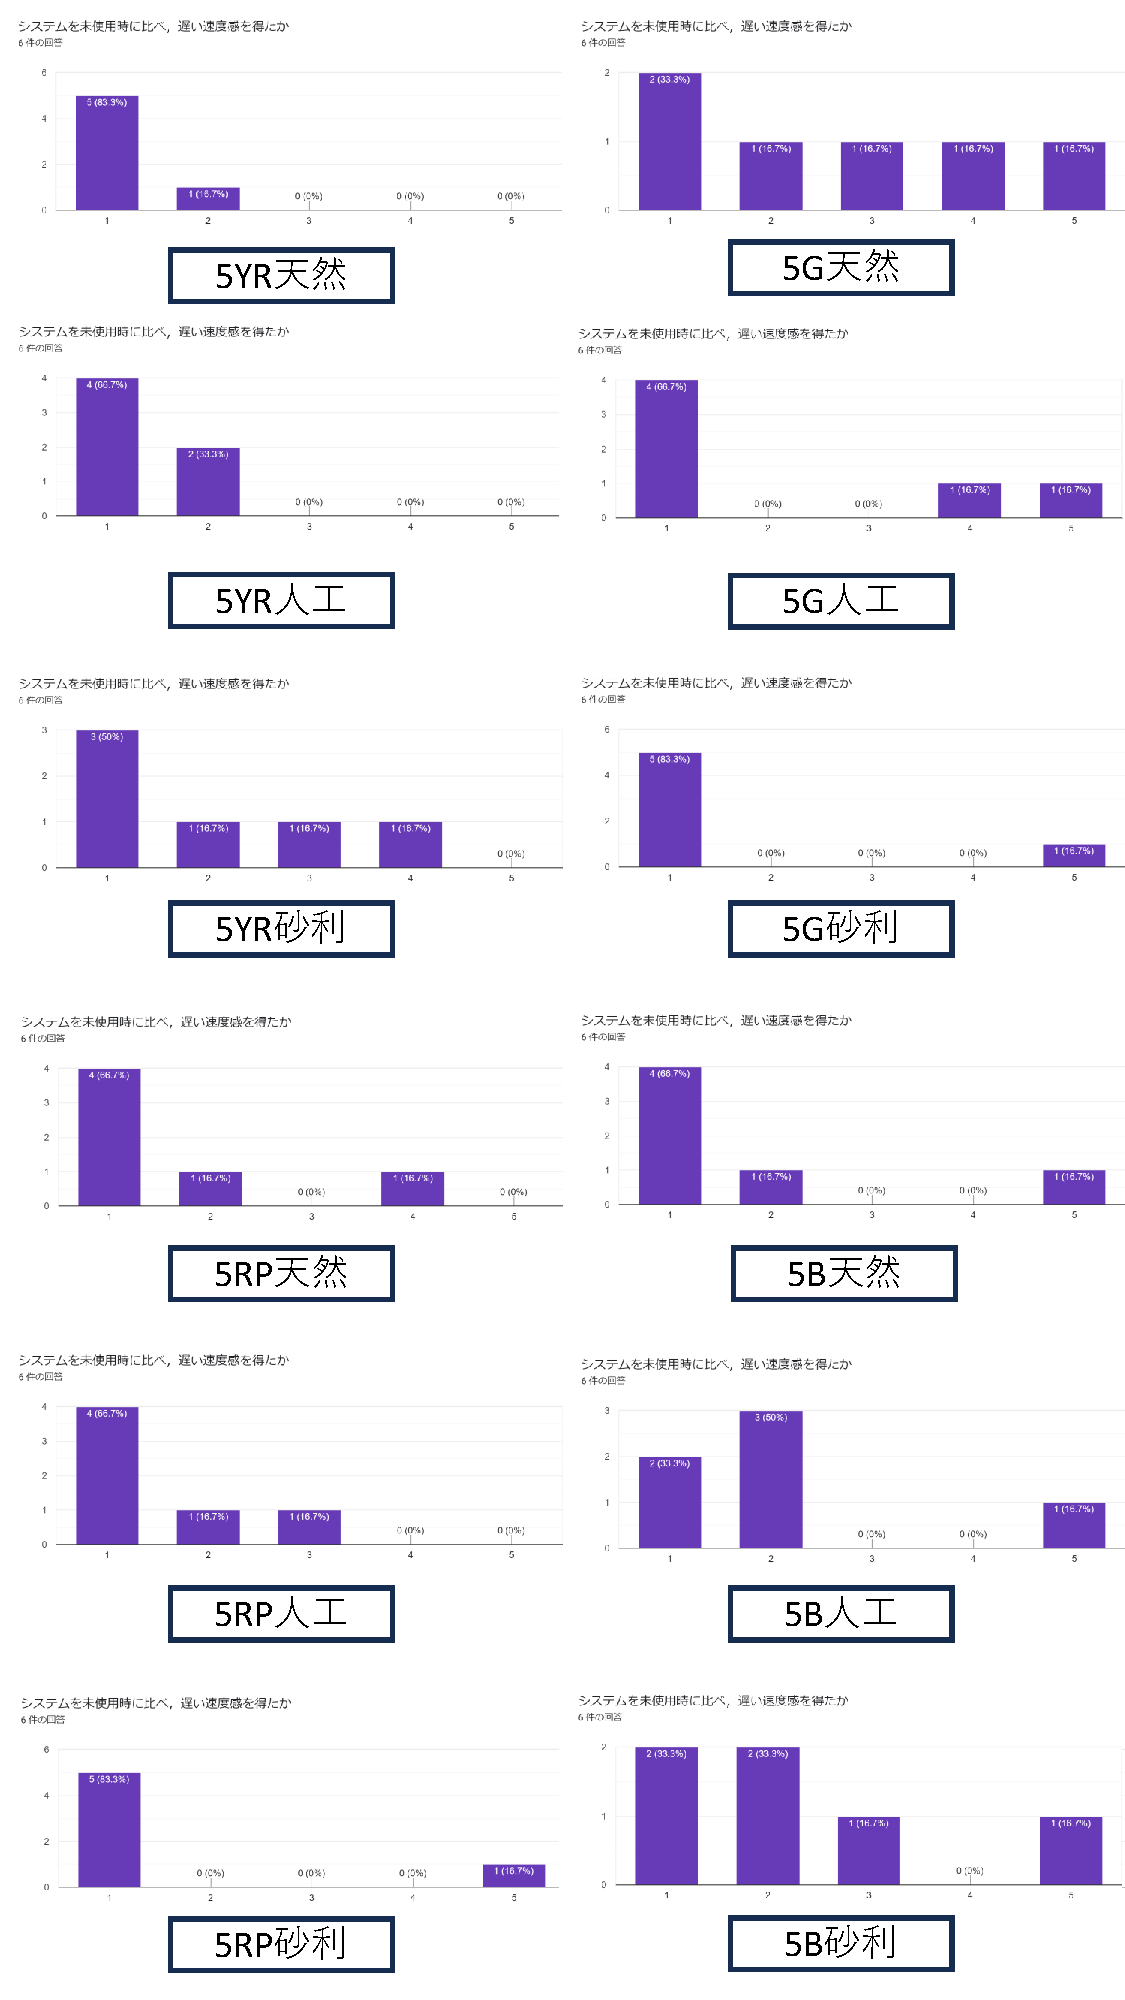
\includegraphics[width=0.7\linewidth]{fig/アンケート結果2.pdf}
    }
    \caption{主観的な速度感に関するアンケート結果(下降)}
    \label{fig:anke2}
\end{figure}

\begin{figure}[H]
    \centering
    \fbox{
        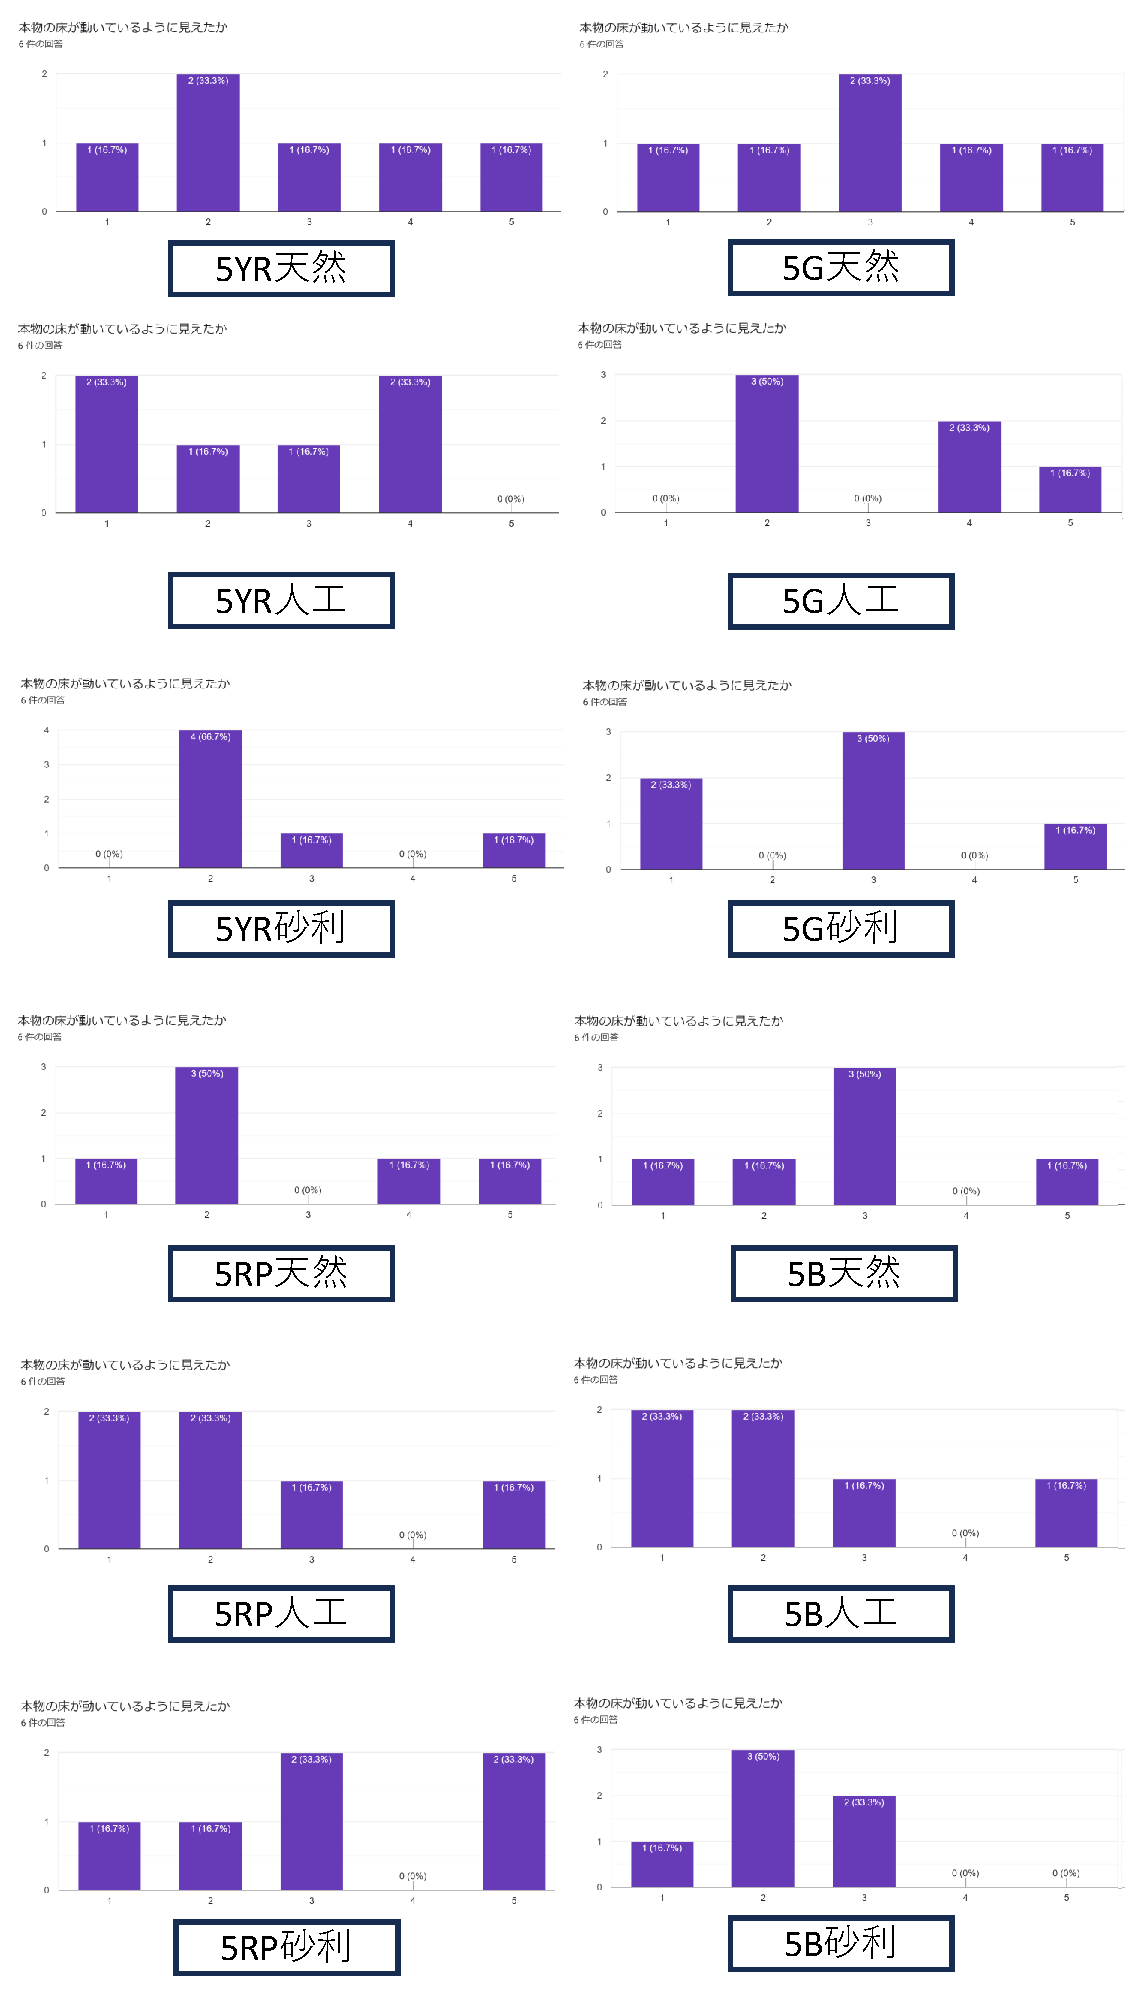
\includegraphics[width=0.7\linewidth]{fig/アンケート結果3.pdf}
    }
    \caption{本物の床が動いているように見えたかのアンケート結果}
    \label{fig:anke3}
\end{figure}




定量評価の結果を以下に示す.
\figref{fig:teiryo}にシステム未使用時とシステム使用時のゴールまでの時間差の一覧を示す.
被験者によって,歩行時間がプラスやマイナスになってしまっている.
また,SSQによる映像酔いの調査結果は上記の評価に対して影響は確認できなかった.
\begin{figure}[H]
    \centering
    \fbox{
        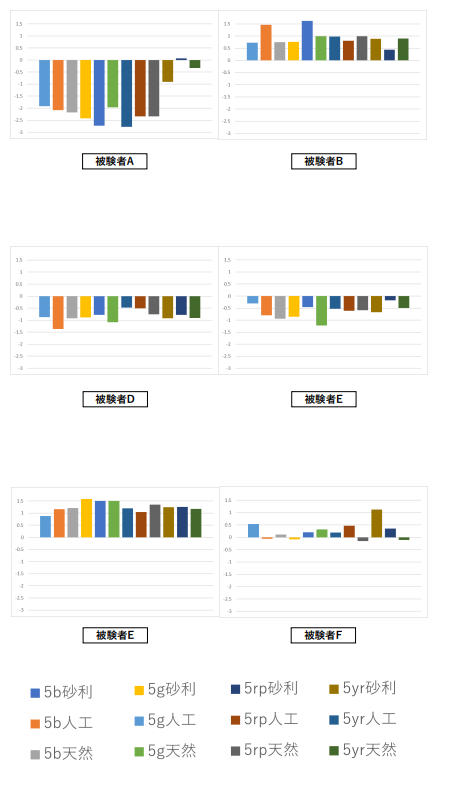
\includegraphics[width=0.7\linewidth]{fig/sokudo.PNG}
    }
    \caption{システム未使用時とシステム使用時のゴールまでの時間差一覧}
    \label{fig:teiryo}
\end{figure}



\section{考察}
定性評価から,今回仮説としてユーザの行動制御ができると考えていたリアルテクスチャは,
現実の床に近似させることは成功したが,
あまり速度感に対する成果ははっきりしなかった.
理由として,「システム未使用時に比べ,速い速度感を得たか」の質問では速度感を得た被験者と得られなかった被験者の数は同数だったことが挙げられる.
このことから,被験者を増やすことでより正確な評価を取る必要があると考える.
コメントでは「目の前で床が消えるので,そこで現実に戻されているような気がする」や
「表示されている床に透明感が強く,実際の床が見え,あまり影響がないように感じた」,「芝が虹色になっている部分がありました」
などの,実験環境の影響によりテクスチャを正確に評価できていない場面もあったため,実験環境を改善する必要があると考えられる.
その他コメントに「速く移動しているようにも感じるし,たくさん移動しているようにも感じた」という意見もあり,
速度感の他に距離感にも影響があると示唆された.

定量評価からは,
どのテクスチャでも有意性を見ることができなかった.
その要因として,実験中の被験者の発言から歩く回数の多さからの疲労や上記のコメントから実験環境に問題があると考えられる.
また,歩行速度が速くなっている被験者と遅くなっている被験者の数はほぼ同じことから,より被験者を増やす必要もあると考える.

また,今回の実験ではバーチャル床が前から被験者に迫ってくる動きを実装したが,後ろから被験者を追い越すように動かすなど,
他のバーチャル床の動きを試すことで別の効果が出るのではないかと考察する.
